\documentclass[../../main]{subfiles}

\renewcommand\thesection{\arabic{section}}


\begin{document}

\section{Cascaded Systems} \label{sec:}

One way to deal with low fidelity models is to cascade it with
a high fidelity model. Figure \ref{fig:cascadingMLModels} shows
such a system.

\begin{figure}
    \centering
    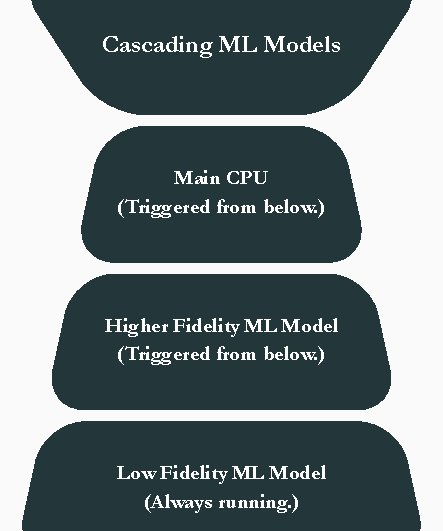
\includegraphics [
        max width = \IGXMaxWidth,
        max height = 0.3\textheight,
        \IGXDefaultOptionalArgs,
    ] {pics/cascading_ml_models.pdf}
    \captionof{figure} {Cascading different fidelity ML models.}
    \label{fig:cascadingMLModels}
\end{figure}

In this case, the low fidelity one will run continuously and consumes
the least amount of energy. Once it picks up something it can wake
up the higher fidelity one to run more inferences. If the higher fidelity
one confirms the lower fidelity one's inferences, then it can trigger
other parts of the system.

In this way, the low fidelity one can help to conserve energy, by preventing
higher fidelity one from running continuously.

\end{document}
